%-----------------------------------------------------------------
% interface_states.tex
%-----------------------------------------------------------------
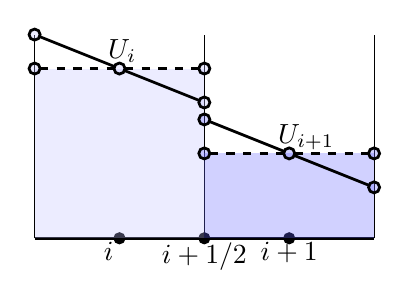
\begin{tikzpicture}[scale = {0.0125\linewidth},
                    inner sep = 1pt,
                    base node/.style={circle,draw,minimum size=4pt}]


% discontinuity
%% \draw[dashed,line width=1pt] (0,0) node[below]{$x_d$} -- (0,0.4); 
%% \draw[-latex,thick](0.05,0.45)node[right]{\small initial discontinuity}
%%          to[out=180,in=90] (0,0.4);

\draw[line width=1pt] (-0.5,0)  -- (-0.25,0) node[below]{$i\phantom{+}$} 
      -- (0,0) node[below]{$i+1/2$}
      -- (0.25,0) node[below]{$i+1$} -- (0.5,0); 

\node[base node,fill=black] at (-0.25,0) {};
\node[base node,fill=black] at (0,0) {};
\node[base node,fill=black] at (0.25,0) {};

\node[shape=circle,fill=black] at (-0.25,0) {};

\draw[] (-0.5,0) -- (-0.5,0.6); 
\draw[] (0,0) -- (0,0.6); 
\draw[] (0.5,0) -- (0.5,0.6); 

% initial states
\fill[blue!25!,opacity=.3] (-0.5,0) rectangle (0,0.5);
\fill[blue!60!,opacity=.3] (0,0) rectangle (0.5,0.25);

\node[base node,fill = blue!25!,opacity=.3] at (-0.5,0.5) {};
\node[base node,line width=1pt] at (-0.5,0.5) {};

\node[base node,fill = blue!25!,opacity=.3] at (-0.25,0.5) {};
\node[base node,line width=1pt] at (-0.25,0.5) {};

\node[base node,fill = blue!25!,opacity=.3] at (0,0.5) {};
\node[base node,line width=1pt] at (0,0.5) {};

\node[base node,fill = blue!60!,opacity=.3] at (0,0.25) {};
\node[base node,line width=1pt] at (0,0.25) {};

\node[base node,fill = blue!60!,opacity=.3] at (0.25,0.25) {};
\node[base node,line width=1pt] at (0.25,0.25) {};

\node[base node,fill = blue!60!,opacity=.3] at (0.5,0.25) {};
\node[base node,line width=1pt] at (0.5,0.25) {};

\draw[dashed,line width=1pt,shorten >= 2 pt, shorten <= 2pt] (-0.5,0.5) -- (-0.25,0.5); 
\draw[dashed,line width=1pt,shorten >= 2 pt, shorten <= 2pt] (-0.25,0.5)  -- (0,0.5); 
\node[above] at (-0.2,0.5) {$\mbf{U}_{i\phantom{-1}}$};

\draw[dashed,line width=1pt,shorten >= 2 pt, shorten <= 2pt] (0,0.25) -- (0.25,0.25); 
\draw[dashed,line width=1pt,shorten >= 2 pt, shorten <= 2pt] (0.25,0.25)  -- (0.5,0.25); 
\node[above] at (0.3,0.25) {$\mbf{U}_{i+1}$};

\draw[line width=1pt,shorten >= 2 pt, shorten <= 2pt] (-0.5,0.6)  -- (-0.25,0.5); 
\draw[line width=1pt,shorten >= 2 pt, shorten <= 2pt] (-0.25,0.5)  -- (0,0.4); 
\node[base node,fill = blue!25!,opacity=.3] at (-0.5,0.6) {};
\node[base node,line width=1pt] at (-0.5,0.6) {};

\node[base node,fill = blue!25!,opacity=.3] at (0,0.4) {};
\node[base node,line width=1pt] at (0,0.4) {};

\draw[line width=1pt,shorten >= 2 pt, shorten <= 2pt] (0,0.35)  -- (0.25,0.25); 
\draw[line width=1pt,shorten >= 2 pt, shorten <= 2pt] (0.25,0.25)  -- (0.5,0.15); 
\node[base node,fill = blue!60!,opacity=.3] at (0,0.35) {};
\node[base node,line width=1pt] at (0,0.35) {};

\node[base node,fill = blue!60!,opacity=.3] at (0.5,0.15) {};
\node[base node,line width=1pt] at (0.5,0.15) {};

% normal
%% \draw[-stealth,thick] (0,0.2) -- (0.1,0.2); 
%% \node[] at (0.05,0.23) {$\hat{n}$};

\end{tikzpicture}
